\documentclass{report}
\usepackage{hyperref,titlesec,tikz,apacite}
\usepackage{fancyhdr}
\pagestyle{fancy}
\fancyhead{}
\fancyfoot{}
\fancyhf{}
\fancyhead[LE,RO]{English report}
\fancyhead[RE,LO]{Made in \LaTeX}
\fancyfoot[CE,CO]{\leftmark}
\fancyfoot[LE,RO]{\thepage}
\titleformat{\chapter}[display]
  {\normalfont\huge\bfseries\filcenter}{\chaptertitlename\ \thechapter}{20pt}{\Huge}
\titlespacing*{\chapter}
  {0pt}{-75pt}{20pt}
\begin{document}
\begin{titlepage}
	\centering
	{\scshape\LARGE Rotterdam University of applied sciences \par}
	{\scshape\LARGE Applied Computer Science \par}
	\vspace{1cm}
	{\huge\bfseries Problems and solutions in the nursing homes\par}
	\vspace{2cm}
	{\Large\itshape Quinten Stekelenburg \par}
	{\Large\itshape 0916193@hr.nl // 0916193 \par}
	{\Large\itshape TI2B \par}
	\vfill
	supervised by\par
	Aninka \textsc{Langras-Rombout}
	Renee \textsc{Van Doorn}

	\vfill

% Bottom of the page
	{\large \today\par}
\end{titlepage}
\tableofcontents{}

\chapter{Introduction}
\thispagestyle{fancy}

During a visit to a nursing home and after speaking to some employees. A few problems surfaced. The largest according to them, is
that they do not have enough time to provide care for the elderly and other people who need nursing.

This is not a 'local' problem according to the CBS (Centraal Bureau voor
de Statistiek). People who work in the health care sector have the
highest workload \cite{CBS2016} . Secondly it is only going to get worse. Due to aging and greying
the Netherlands now counts 3,085,308 elderly (people who are 65+) \cite{CBSBevolking}. And
in the following years this will increase with around 1,500,00 to 4,5
million elderly \cite{CBSPrognose2014} . And with 1,400,00 nurses taking care of everyone,
everything has to be on a tight schedule. And that means that there is
no room for a social chat with the elderly, or any mistake in terms of walking to the incorrect room or bringing the wrong gear.

During the interview with the nurses, they said that they have to do a lot of paperwork. And when they do their paperwork, they cannot take care of someone. The systems in place for scheduling and
paying the nurses, is flawed and hard to use.

And this is where the solution comes in. iCCs is a revolutionary
framework that will facilitate all the different
programs/apps/applications that the nurse needs. No longer do they need
to manually enter their schedule in a different program, it will
automatically be exported to all the systems that need it. The medicine list cannot be found? No worries, it is right there on their phone.

\chapter{The revolution named iCCs}
\thispagestyle{fancy}

As mentioned in the introduction the solution to the problems of having a high workload and flawed ICT-systems is iCCs. In this chapter the explanation can be found on why this system is revolutionary, and why it is a benefit to your organization.

\section{What does iCCs stand for?}

iCCs, is short for Integrated Collapsed Care System. This application will replace, or inherit all the other ICT-systems in the nursing home. And because it will have inherited every system, it is automatically integrated in your nursing home. It will also guarantee the most productive and efficient interaction with ICT. It is also a framework, which means that the applications implemented in iCCs will be able to exchange data.


\section{What can iCCs bring to your organization}

Less time doing paperwork, and more time spend with your clients. During the interview with the nursing staff at Huis aan de Vecht a problem surfaced, they have to make the work schedule twice. Since the schedule is first made in excel using colours and letters. And then manually exported to a DRP (Distribution Requirements Planning). In iCCs, employees will never have to do the same work twice. Since everything the nurses make or put in to the framework will automatically be shared with any other application that might need that information. 

Furthermore, the work schedule is printed and placed in the office of the nurses. But what happens when a member of the staff forgets his or her schedule? With iCCs there is no problem, the staff member can just grab his or her smartphone and login to iCCs. And check the schedule while roaming the halls of the nursing home.

\subsection{Functions of iCCs}

In addition to a schedule and payout system. iCCs will also support parking using an application similair to Parkline. The system will also be able to contain patient files, and other useful information on clients. When the smartphone has a NFC-chip(short range transmitter/receiver), iCCs also will be able to store access passes.
Privacy is an important factor in the health care, therefor iCCs will have the latest security standards that are available. Employees will not be able to make screenshots of the data of patients seen on their phone. Digital communication will be encrypted, so data does not get leaked. 

\chapter{The framework that bring innovation to the nursing home}
\thispagestyle{fancy}

iCCs is innovative because no one has ever even tried to combine all of the ICT-systems into one system. And also because it will be the most simple system ever. This product needs to be quick and easy to use, as to boost the efficiency and productivity in nursing homes. Because when a system is capable of doing everything an employee needs, most of the times this will be a complex system. But not in the case of iCCs. This system will be easy to use for everyone, and this is necessary. According to a study to the effects of using a DRP-system. If employees do not know how to use the system, the system will be pushed aside and the employees will work as they always did \cite{Michels2009}.It is useless if the nursing home has a bad ICT-infrastructure. Furthermore the study says that when implemented correctly, it will lead to a correct work load distribution. Nowadays employees who regularly work heavy shifts, will continue to keep working those. When iCCs is implemented, all the work load will be distributed in a way that all the employees will work evenly heavy shifts.
  
\chapter{How can iCCs benefit your organization?}
\thispagestyle{fancy}
\section{Pros}

The system will be built in a way that everyone can use it, without needing a high investment in learning to operate the system. iCCs will combine all the strengths of the ICT-systems, to create an application that everyone can use. This system will relieve work load from the nurses, so they can spend more time with clients and thus provide better care\cite{Michels2009). The offices used for other activities than taking care of clients, will be mostly empty. Because this system provides a quicker way to take care of the paperwork that nowadays prevents nurses to nurse.

This ICT-solution will be setup in a way that only higher ranking employees can adjust the schedule. Not all employees will have the rights to edit/change the system, because that means chaos. 

iCCs will be available on desktops, for example to create the work schedules. It will also feature an android application, so that a nurse can check his/her work schedule while roaming the nursing home. 

Furthermore all data send/received and available in the program will be encrypted, as to ensure client and employee privacy. When someone wants to login to iCCs, they will need a username and password. By this the management can 'track' your employees, but also keep bad people out of your system\cite{Florencio2007}.

If the smartphone has a NFC-chip, the smartphone also will be able to store keycards. This in turn means that an employee can use the phone to gain access to the nursing home, instead of the keycard\cite{dragani2014}. 

\section{Cons}

The reception of this product will probably be negative, as most employees will be hesitant to use this system. Because after all this is yet another system to make their lives easier. So when this system is distributed and implemented in the nursing homes, there needs to be a campaign on why this system does work\cite{Michels2009}. 

Furthermore the system will need servers and other hardware, not all nursing homes have enough budget to make that happen. 

And because this is a system with a lot of options, it will difficult to make it accessible and easy to use for everyone. So a lot of this product's resources need to go to research, in how to create the most user-friendly system. Work schedules need to be understood by the developers creating this solution, because this product needs to fit seamlessly in the organization. And so is the case for every other application that will be implemented in iCCs. 

\chapter{Conclusion}
\thispagestyle{fancy}

There are some major problems in the health care sector, one of them is nurses using the much needed care-time to fill out paperwork. iCCs will be a solution to this problem. It is a revolutionary framework that implements all the applications/systems/apps the nurse needs. It will prevent doing work double, so that the nurses have more time to take care of the clients. And this is needed as more and more people reach old age, and nurses are in low supply. 

The system needs to succeed where others fail. Most of the systems used nowadays are hard to understand, or do not boost productivity and efficiency. This framework will be available across all platforms, so nurses always have the needed information on hand. iCCs will be easy to understand, as the most nurses do not possess advanced technical insight. 

Acquiring this system as an organization will be an investment, but it will be useful in the long run. The system will have state of the art security, to ensure the privacy of everyone in the nursing home. There needs to be invested in ICT-infrastructure, but also in researching the work flows in a nursing home. 

Opposing the investments are great pros. One system to rule them all, lower workload, happier nurses and of course more time for the clients who need care.
\vfill

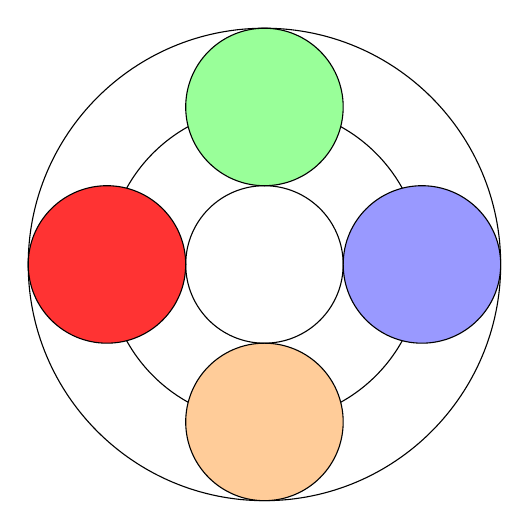
\begin{tikzpicture}
	\draw (2,2) circle (3cm);
	\draw (2,2) circle (2cm);
	\draw (2,2) circle (1cm);
	\filldraw[fill=red!80!white, draw = black] (0,2) circle (1cm);
	\filldraw[fill=orange!40!white, draw = black] (2,0) circle (1cm);
	\filldraw[fill=green!40!white, draw = black] (2,4) circle (1cm);
	\filldraw[fill=blue!40!white, draw = black] (4,2) circle (1cm);
\end{tikzpicture}}

\bibliographystyle{apacite}
\bibliography{library}
\end{document}